\documentclass[tikz,border=3pt]{standalone}
\usepackage[utf8]{inputenc}
\usepackage[T1]{fontenc}
\usepackage{lmodern}
\renewcommand{\familydefault}{\sfdefault}
\usepackage{sansmath}\sansmath
\usepackage{pgfplots}\pgfplotsset{compat=1.18,/pgf/number format/use comma,/pgf/number format/1000 sep={.}}
\usetikzlibrary{arrows.meta,calc,positioning,decorations.pathmorphing,patterns}
% paleta del sitio
\definecolor{nar}{HTML}{E8680C}\definecolor{narc}{HTML}{FFB35C}\definecolor{hielo}{HTML}{FFF3E8}
\definecolor{tinta}{HTML}{1D1D1F}\definecolor{gris}{HTML}{6E6E73}\definecolor{lila}{HTML}{7C5CF0}
\definecolor{azul}{HTML}{2F6FD6}\definecolor{menta}{HTML}{17A673}\definecolor{coral}{HTML}{E8342A}
\begin{document}
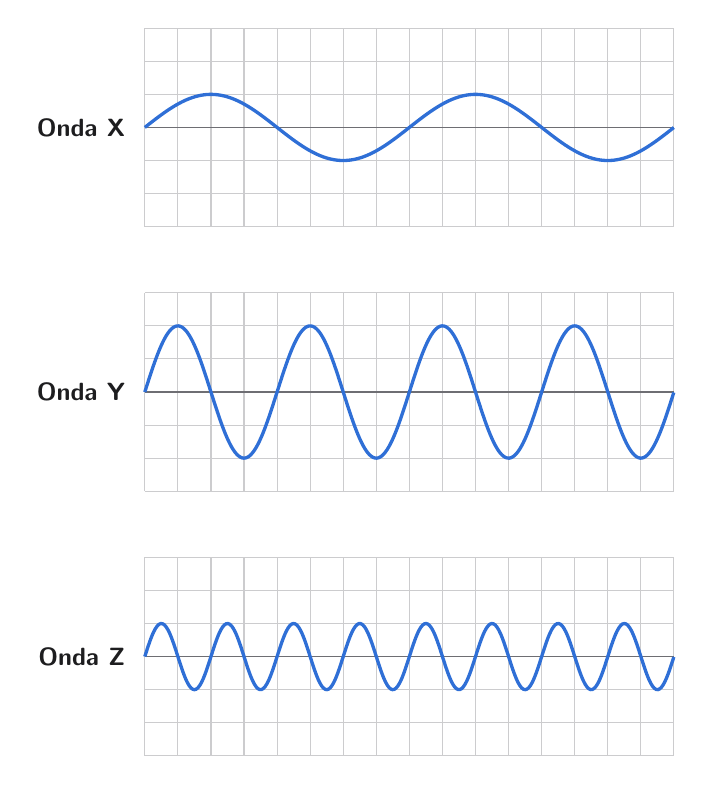
\begin{tikzpicture}[font=\footnotesize,>={Stealth[length=2.4mm]}]
\begin{scope}[scale=0.42]
\foreach \yo/\nom/\lam/\amp in {0/X/8/1, -8/Y/4/2, -16/Z/2/1}{
  \begin{scope}[yshift=\yo cm]
  \draw[gris!35,step=1] (0,-3) grid (16,3);
  \draw[gris,thin] (0,0) -- (16,0);
  \draw[very thick,azul,domain=0:16,samples=300,smooth] plot (\x,{\amp*sin(360*\x/\lam)});
  \node[left,font=\small\bfseries,text=tinta] at (-0.3,0) {Onda \nom};
  \end{scope}}
\end{scope}
\end{tikzpicture}
\end{document}
